% Compile using LuaLaTeX!

\documentclass{beamer}

% Beamer
\usetheme{Warsaw} % or split
\usecolortheme{grass}
\setbeamercovered{transparent}
% Navigation ausblenden
\setbeamertemplate{navigation symbols}{}%remove navigation symbols

% Zeilenabstand verringer
\renewcommand{\baselinestretch}{0.9}

% more flexible than babel. Requires LuaLaTeX or XeTeX
\usepackage{polyglossia}
\setdefaultlanguage{german}

% LuaTeX and XeTeX (but LuaLaTeX is cooler) -> fontspec
\usepackage{fontspec}

% extra symbols
\usepackage{amsmath}
\usepackage{amsfonts}
\usepackage{amssymb}
\usepackage{amsthm}

\usepackage{multimedia}

\usepackage{hyperref}
% Hyperref Optionen - makeatletter/AtBeginDocument erlaubt uns Titel/Author dynamisch zu setzen, wenn gewollt
\makeatletter
\hypersetup{
	unicode = true,
	pdftoolbar = true,
	pdfmenubar = true,
	pdffitwindow = true,
	pdftitle = {\@title},
	pdfauthor = {\@author},
	pdfsubject = {PING e.V. und FOSS-AG},
	colorlinks = true,
	linkcolor = black,
	citecolor = black,
	filecolor = black,
	urlcolor = black
}
\makeatother

\usepackage[]{graphicx}
\graphicspath{{../resources/}}
\usepackage{listings}
\usepackage{pdfpages}
\usepackage{color}
\definecolor{tuGreen}{rgb}{0.517,0.721,0.094}
\definecolor{tuOrange}{rgb}{1.0,0.7176,0.0}
\definecolor{brightGray}{gray}{0.9}
\definecolor{darkGray}{gray}{0.2}
\definecolor{white}{rgb}{1,1,1}
\definecolor{black}{rgb}{0,0,0}
\definecolor{red}{rgb}{1,0,0}


% Abkuerzungen richtig formatieren
\usepackage{xspace}
\newcommand{\vgl}{vgl.\xspace} 
\newcommand{\zB}{z.\,B.\xspace}
\newcommand{\dahe}{d.\,h.\nolinebreak[4]\xspace}
\newcommand{\uvm}{u.\,v.\,m.\xspace}
\newcommand{\usw}{u.\,s.\,w.\xspace}
\newcommand{\sg}{s.\,g.\xspace}
\newcommand{\iA}{i.\,A.\xspace}
\newcommand{\sa}{s.\,a.\xspace}
\newcommand{\su}{s.\,u.\xspace}
\newcommand{\ua}{u.\,a.\xspace}
\newcommand{\og}{o.\,g.\xspace}
\newcommand{\oae}{o.\,\"a.\xspace}
\newcommand{\oBdA}{o.\,B.\,d.\,A.\xspace}
\newcommand{\OBdA}{O.\,B.\,d.\,A.\xspace}

% footnote ohne marker blfootnote
\newcommand\blfootnote[1]{%
	\begingroup
	\renewcommand\thefootnote{}\footnote{#1}%
	\addtocounter{footnote}{-1}%
	\endgroup
}


\author{
	PING e.V.
	\and \\
	FOSS-AG
}
\date{\today}

\subject{Einladung}
\title{Einladung: Linux Days Dortmund 2017}
\subtitle{\textcolor{black}{P}rivate \textcolor{black}{I}nternet \textcolor{black}{N}utzer \textcolor{black}{G}emeinschaft und \textcolor{black}{F}ree and \textcolor{black}{O}pen \textcolor{black}{S}ource \textcolor{black}{S}oftware \textcolor{black}{- AG}}

\begin{document}	
	\begin{frame}
		\begin{center}
			\hspace{-0.9cm}\begin{minipage}{0.12\linewidth}
				
\includegraphics[scale=0.1]{tux}
			\end{minipage}
			\begin{minipage}{0.9\linewidth}
				{\scriptsize Der PING e.V. Dortmund in Kooperation mit der FOSS-AG TU-DO lädt ein:}
				\begin{minipage}{0.01\linewidth}
					
\includegraphics[scale=0.1]{tux}
				\end{minipage}
			\end{minipage}
			
			\vspace{0.2cm}
			{\large \textbf{Linux Days Dortmund 2017}}
		\end{center}
	
		\vspace{0.2cm}
		\begin{minipage}{0.56\linewidth}
			\begin{itemize}
				\item[Wann?] \textbf{24.06.17} ab 12:00 Uhr \\
				\textbf{25.06.17} ab 12:30 Uhr\\
				\textbf{01.07.17} ab 12:00 Uhr
				\item[Wo?] PING e.V. \textbf{Zum Nubbental 11}, 44227 Dortmund
				\item[Infos:] \textbf{www.foss-ag.de}
				\item[] Natürlich kostenlos!
			\end{itemize}
		\end{minipage}
		\begin{minipage}{0.35\linewidth}
			{\scriptsize \hspace{0.03cm} PING Vereinsheim: \\ }
			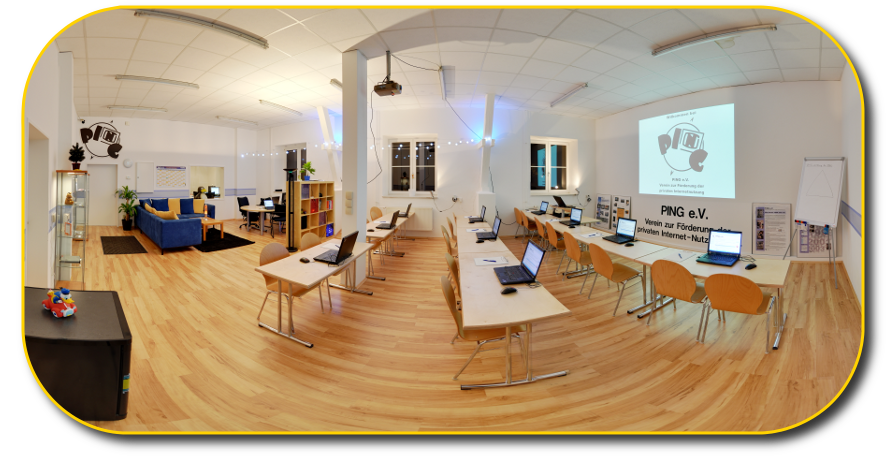
\includegraphics[scale=0.37]{weiterbildung-schulungsraum}
		\end{minipage}
	
		\vspace{0.5cm}
		Was wird geboten?
	
		{ \scriptsize
			\begin{minipage}{0.56\linewidth}
				\begin{itemize}
					\item Einführung in die Themen Free-/Open-Source und Linux
					\item Offene und lockere Diskussionsrunden
					\item Hands-on: Linux, Terminal, Scripting
					\item Lecker, lecker was vom Grill!
				\end{itemize}
			\end{minipage}
		}	
		\begin{minipage}{0.35\linewidth}
			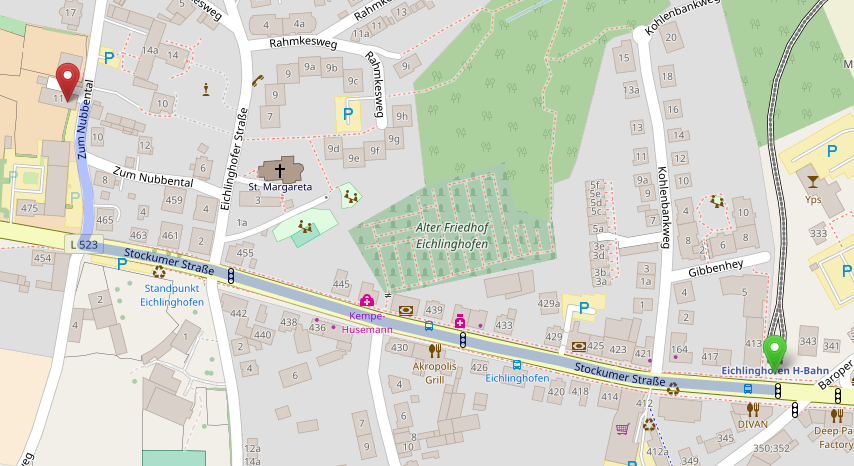
\includegraphics[scale=0.23]{map}
		\end{minipage}
	\end{frame}
\end{document}